\documentclass[class=report, crop=false, 12pt,a4paper]{standalone}
\usepackage{enumitem}
\usepackage{multicol}
\usepackage{graphicx}
\usepackage{float}
\usepackage{amsmath}
\usepackage{amssymb}
\usepackage{mathtools}
\usepackage{siunitx}
\usepackage{commath}
\usepackage{array}
\usepackage{natbib}
\usepackage[a4paper,width=150mm,top=25mm,bottom=25mm]{geometry}
\setlength{\parindent}{0pt}
\begin{document}
\section{Module Introduction}
\subsection{Teaching Team}
\begin{itemize}
	\item Dr Gemma Cremen - Lecture in Resilience Engineering, Module Coordinator
	      \begin{itemize}
		      \item g.cremen@ucl.ac.uk
	      \end{itemize}
	\item Dr Tim Hillel - Lecturer in Analytics of Infrastructure Systems, Deputy Module Coordinator
	      \begin{itemize}
		      \item tim.hillel@ucl.ac.uk
	      \end{itemize}
	\item Mr Umut Lagap - PhD Student in Risk and Resilience, PGTA
	      \begin{itemize}
		      \item umut.lagap.21@ucl.ac.uk
	      \end{itemize}
\end{itemize}
\subsection{Assessment}
\begin{figure}[H]
	\centering
	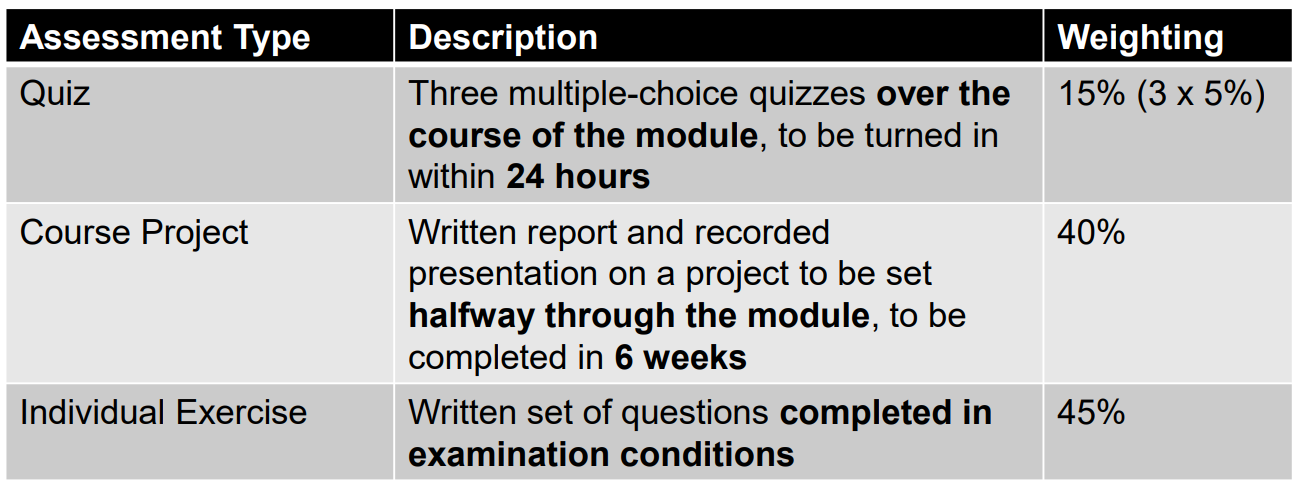
\includegraphics[width = 0.9 \textwidth]{../img/figure1.png}
	\caption{Module Assessment.}
\end{figure}
\subsection{Timeline}
\begin{figure}[H]
	\centering
	
\includegraphics[width = 0.9 \textwidth]{../img/figure2.png}
	\caption{Module Timeline.}
\end{figure}
\section{Introduction and overview of mixed economies}
\subsection{Aims}
\begin{enumerate}
	\item Understand the roles of the private and public sector in mixed economies
	\item Become (re)familiar with key microeconomic concepts of consumption and production, including Pareto optimality and market equilibrium
	\item Understand the trade-offs between market efficiency and equitable distribution of resources
	\item Be aware of the assumptions and limitations of fundamental theorems and associated neoclassical economics
\end{enumerate}
\subsection{Economies}
\subsubsection{A simplified definition}
\begin{quote}
	An area of \textit{production, trade} and \textit{consumption} of goods and services by different \textit{agents}.
\end{quote}
\subsubsection{Agents}
\begin{itemize}
	\item Individuals and households
	\item Businesses
	\item Government
\end{itemize}
\subsection{Mixed economies}
\subsubsection{Economies today are predominantly \textit{mixed economies}}
Private sector:
\begin{quote}
	profit-maximising firms operate in competitive markets
\end{quote}
Public sector:
\begin{quote}
	governments/other organisations make interventions in those markets
\end{quote}
\subsection{Private sector}
\subsubsection{Welfare economics}
\begin{quote}
	"he is in this, as in many other cases, led by an invisible hand to promote an end which has no part of his intention. Nor is it always the worse for the society that it was no part of it. By pursuing his own interest he frequently promotes that of the society more effectively than when he really intends to promote it. (Smith 1776)
\end{quote}
\subsection{Public sector}
\subsubsection{Public sector aims to balence trade-offs}
In particular
\begin{quote}
	efficiency of competitive markets vs. improved equity of distribution of income from regulation
\end{quote}
Understanding the role of public sector in mixed economies first requires u s to understand operation of free-markets
\subsection{Classical microeconomics}
\begin{figure}[H]
	\centering
	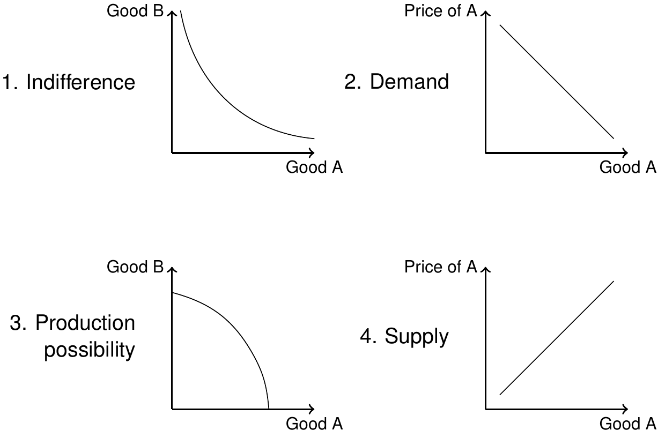
\includegraphics[width = 0.9 \textwidth]{../img/figure3.png}
	\caption{Classical microeconomic models.}
\end{figure}
\subsection{Economic models}
\begin{quote}
	"Remember that all models are wrong; the practical question is how wrong do they have to be to not be useful" (Box and Draper 1987)
\end{quote}
\section{Consumer theory}
\subsection{Consumer theory: continuous goods}
\begin{itemize}
	\item $J$ continuous goods, each good denoted by $j = 1, \, ..., \, J$
	\item Each good has associated price per unit $p_j$
	      \begin{itemize}
		      \item e.g., $j = 1$ corresponds to milk, $p_j = \SI{90}{pence\per litre}$
		      \item $j = 2$ corresponds to eggs, $p_j = \SI{16}{pence \per egg}$
	      \end{itemize}
	\item Consider choice of agent, with total budget $I$
	      \begin{itemize}
		      \item Assume agent represents individual
		      \item Individual chooses quantity $q_j$ of each good $j$, subject to budget constraint
	      \end{itemize}
\end{itemize}
\begin{gather}
	\sum_{j=1}^{J} \left(p_jq_j\right) \leq I
\end{gather}
\subsection{Utility}
\begin{itemize}
	\item Individual's choice of goods represented by consumption bundle $Q$
	      \begin{itemize}
		      \item i.e. vector of $q_1, \, ..., \, q_J$
	      \end{itemize}
	\item Individual gets utility $U\left(Q\right)$ from $Q$
	      \begin{itemize}
		      \item Utility represents how individuals perceived benefit from consuming/owning $Q$
		      \item Assume $U\left(Q\right)$ increases monotonically with increasing $q_i$
	      \end{itemize}
\end{itemize}
\subsection{Choice between two continuous goods}
\begin{figure}[H]
	\centering
	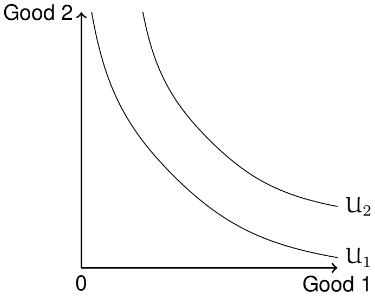
\includegraphics[width = 0.5\textwidth]{../img/figure4.png}
	\caption{}
\end{figure}
Indifference curves:
\begin{quote}
	Different combinations of each good that yield same level of utility
\end{quote}
Marginal Rate of Substitution (MRS):
\begin{quote}
	Gradient of indifference curve
\end{quote}
\begin{itemize}
	\item i.e. how many unites of good 2 individual would substitute for 1 unit of good 1
	\item Assumed to be convex
\end{itemize}
\subsection{Utility maximisation with budget constraint}
\begin{figure}[H]
	\centering
	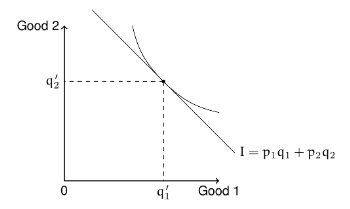
\includegraphics[width = 0.5\textwidth]{../img/figure5.png}
	\caption{}
\end{figure}
\begin{itemize}
	\item Assume agents try to maximise utility
	\item Under maximal utility assumption, optimal solution when indifference curve is tangent to budget line
\end{itemize}
\begin{gather}
	\textrm{MRS} = \dfrac{p_1}{p_2}
\end{gather}
\subsection{Trade between two agents}
\begin{figure}[H]
	\centering
	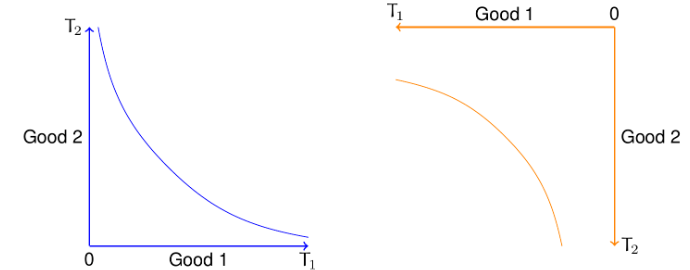
\includegraphics[width = \textwidth]{../img/figure6.png}
	\caption{}
\end{figure}
\subsection{Edgeworth box}
\begin{figure}[H]
	\centering
	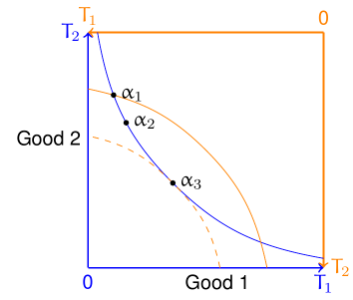
\includegraphics[width =0.5 \textwidth]{../img/figure7.png}
	\caption{}
\end{figure}
Edgeworth box:
\begin{quote}
	depicts distribution of commodities in closed economy between two agents
\end{quote}
Pareto improvement:
\begin{quote}
	A reallocation that improves utility of of one individual without reducing anyone else's utility
\end{quote}
\begin{itemize}
	\item $\alpha_2$ is Pareto improvement of $\alpha_1$
	\item $\alpha_3$ is Pareto improvement of $\alpha_2$
\end{itemize}
Pareto optimal/efficient:
\begin{quote}
	An allocation from which no-one can improve utility without reducing someone else's
\end{quote}
\begin{itemize}
	\item $\alpha_3$ is Pareto optimal
\end{itemize}
\subsection{Pareto efficiency}
\begin{itemize}
	\item Pareto efficient solutions happen when indifference curves have equal gradient
	\item i.e. each agent has equal MRS
\end{itemize}
Pareto frontier:
\begin{quote}
	Set of all possible Pareto efficient allocations
\end{quote}
\section{Producer theory}
\subsection{Production of goods and services}
\begin{figure}[H]
	\centering
	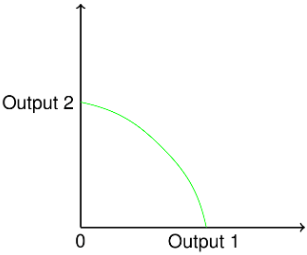
\includegraphics[width =0.5 \textwidth]{../img/figure8.png}
	\caption{}
\end{figure}
Production Possibilities Frontier (PPF):
\begin{quote}
	possible combinations of outputs (e.g. goods/services) that can be produced by economy with fixed inputs technology
\end{quote}
\begin{itemize}
	\item all points on PPF are production efficient: no more of one output can be produced without sacrificing the other
\end{itemize}
Marginal Rate of Transformation (MRT):
\begin{quote}
	Gradient of PPF
\end{quote}
\begin{itemize}
	\item Measures amount of Output 2 that must be sacrificed to produced additional unit of Output 1
\end{itemize}
\subsection{Marginal cost}
\begin{figure}[H]
	\centering
	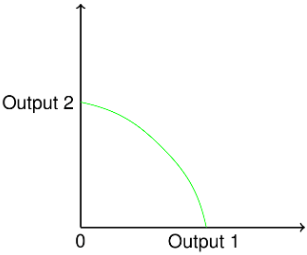
\includegraphics[width =0.5 \textwidth]{../img/figure8.png}
	\caption{}
\end{figure}
Marginal cost:
\begin{quote}
	Cost of producing one additional unit of output
\end{quote}
\begin{gather}
	\textrm{MRT} = \dfrac{MC_{output_1}}{MC_{output_2}}
\end{gather}
\begin{itemize}
	\item PPF often assumed to be concave under certain conditions (i.e. rewards diversity)
	      \begin{itemize}
		      \item Easier to obtain low-hanging fruit
	      \end{itemize}
\end{itemize}
\subsection{Pareto efficient production}
\begin{figure}[H]
	\centering
	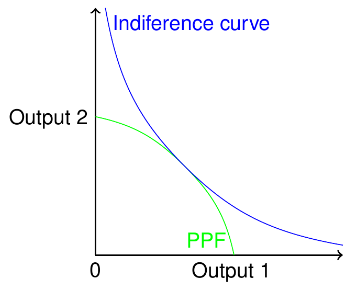
\includegraphics[width =0.5 \textwidth]{../img/figure9.png}
	\caption{}
\end{figure}
Pareto efficiency only achieved when production of goods matches consumers' willingness to pay
\begin{itemize}
	\item Gradient of PPF matches combined indifference curve of all consumers
	\item i.e. MRS = MRT
\end{itemize}
\subsection{Single market efficiency}
\begin{figure}[H]
	\centering
	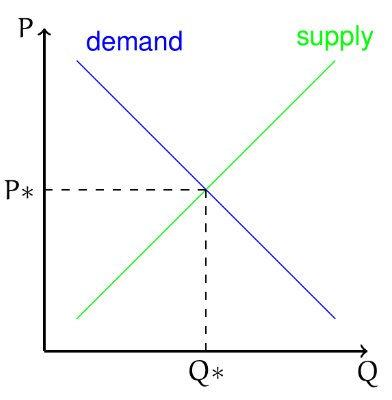
\includegraphics[width =0.5 \textwidth]{../img/figure10.png}
	\caption{}
\end{figure}
Market equilibrium occurs when supply equals demand
\begin{itemize}
	\item marginal benefit of consumption is equal to marginal cost of production
\end{itemize}
\section{Fundamental theorems of welfare economics}
\subsection{Competitive economies}
\subsubsection{Fundamental theorems of welfare economics}
If the economy is competitive, it is Pareto efficient
\subsection{Efficiency vs equality}
\begin{figure}[H]
	\centering
	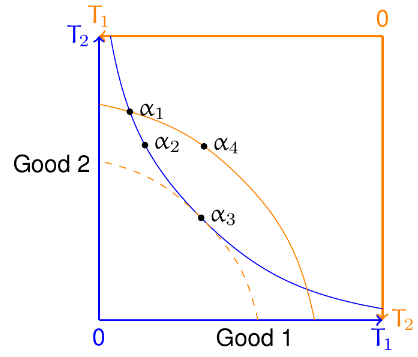
\includegraphics[width =0.5 \textwidth]{../img/figure11.png}
	\caption{}
\end{figure}
\begin{itemize}
	\item So far, considered only efficiency of allocations
	      \begin{itemize}
		      \item $\alpha_3$ is Pareto efficient
	      \end{itemize}
	\item Social welfare also depends on equitable distribution of goods
	\item How do we choose between $\alpha_3$ and $\alpha_4$
	      \begin{itemize}
		      \item Do we need to?
	      \end{itemize}
\end{itemize}
\subsection{Wealth distribution}
\subsubsection{Fundamental theorems of welfare economics}
\begin{itemize}
	\item If the economy is competitive, it is Pareto efficient
	\item Every Pareto efficient resource allocation can be obtained with competitive market process with an appropriate initial redistribution of wealth
\end{itemize}
\subsection{Efficiency and equality?}
\begin{figure}[H]
	\centering
	
\includegraphics[width =0.5 \textwidth]{../img/figure12.png}
	\caption{}
\end{figure}
According to second fundamental theorem:
\begin{quote}
	more equitable allocation can be found through suitable assignment of initial endowments and free trade
\end{quote}
\section{Public sector}
\subsection{Role of government: the theory}
\subsubsection{When and how should governments make interventions in mixed economies?}
According to first fundamental theorem:
\begin{quote}
	government interventions that reduce competition make economies less efficient
\end{quote}
\begin{quote}
	Redistribute income and leave markets alone?
\end{quote}
\subsection{Role of government: reality}
Note\dots Governments play an active role in all major economies, including:
\begin{itemize}
	\item Allocation
	\item Distribution
	\item Regulation
	\item Stabilisation
\end{itemize}
\subsection{Market failures}
Several situations result in the failure of free markets to achieve optimal solutions. Causes include:
\begin{itemize}
	\item existence and need for public goods
	\item existence of externalities
	\item imperfect competition
	\item incomplete information and uncertainty
\end{itemize}
\section{Review and recap}
\subsection{A need for better understanding?}
\begin{itemize}
	\item Several strong assumptions
	      \begin{itemize}
		      \item Individuals as rational utility maximisers
		      \item Equivalence of utility, value and price
		      \item Markets as continuous
		      \item Statics tastes and preferences
		      \item Perfect competition
	      \end{itemize}
	\item Fundamental welfare economic theory does not capture
	      \begin{itemize}
		      \item unpaid labour
		      \item social exchange
		      \item long-term resilience and sustainability
	      \end{itemize}
\end{itemize}
\end{document}